% p10-05 引入：矩形 ABCD AB=8 AD=6，沿对角线 BD 折 △ABD 至 △A'BD
% B(0,0), C(8,0), D(8,6), A(0,6)
% A' = 2H - A，其中 H 为 A 在 BD 上的投影
% BD: 从 (0,0) 到 (8,6)，长 10；单位 u=(0.8,0.6)；A-B=(0,6)；投影长 = 0*0.8+6*0.6 = 3.6
% H = 3.6*(0.8,0.6) = (2.88, 2.16)；A' = 2H - A = (5.76, -1.68)
\documentclass[tikz,border=4pt]{standalone}
\usepackage{ctex}
\usepackage{amsmath}
\usetikzlibrary{calc}
\begin{document}
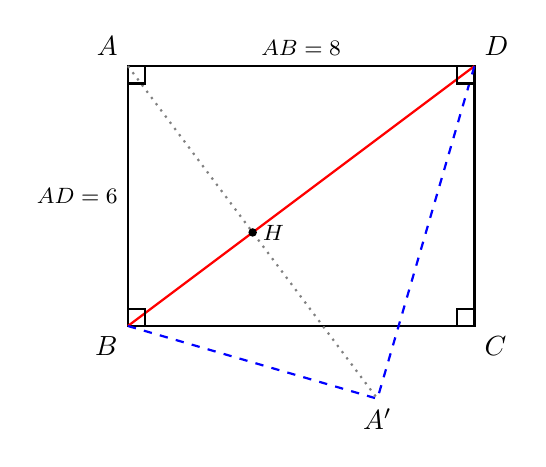
\begin{tikzpicture}[scale=0.55, thick]
  \coordinate (B) at (0,0);
  \coordinate (C) at (8,0);
  \coordinate (D) at (8,6);
  \coordinate (A) at (0,6);
  \coordinate (H) at (2.88, 2.16);
  \coordinate (Ap) at (5.76, -1.68);

  \draw (B)--(C)--(D)--(A)--cycle;
  \draw[red] (B)--(D);                       % 折痕
  \draw[blue, dashed] (B)--(Ap)--(D);        % 折后 △A'BD
  \draw[gray, dotted] (A)--(Ap);

  \filldraw (H) circle (2pt);

  % 直角符号
  \draw ($(B)+(0.4,0)$)--($(B)+(0.4,0.4)$)--($(B)+(0,0.4)$);
  \draw ($(A)+(0.4,0)$)--($(A)+(0.4,-0.4)$)--($(A)+(0,-0.4)$);
  \draw ($(C)+(-0.4,0)$)--($(C)+(-0.4,0.4)$)--($(C)+(0,0.4)$);
  \draw ($(D)+(-0.4,0)$)--($(D)+(-0.4,-0.4)$)--($(D)+(0,-0.4)$);

  \node[above left]  at (A) {$A$};
  \node[below left]  at (B) {$B$};
  \node[below right] at (C) {$C$};
  \node[above right] at (D) {$D$};
  \node[below] at (Ap) {$A'$};
  \node[right] at (H) {\footnotesize $H$};

  \node[above] at ($(A)!0.5!(D)$) {\footnotesize $AB=8$};
  \node[left]  at ($(A)!0.5!(B)$) {\footnotesize $AD=6$};
\end{tikzpicture}
\end{document}
